\chapter{Results}
\label{chap:results}
We expect that the \gls{wdt} method will improve the statistics of
Serpent 2 calculations. With normal delta-tracking, virtual collisions
provide no statistical benefit, and are therefore an inefficient use
of computational resources. Virtual collisions that results in
absorption events do contribute to statistics when using
\gls{wdt}. Therefore, we expect an improvement in the results of a
Serpent 2 simulation. In this section, we will describe how
performance in Serpent 2 is quantified, describe the three test cases,
and the results of those test cases.

\section{Performance metrics}
\label{sec:fom}

\subsection{Figure of Merit}
\label{sec:fom}

Monte Carlo codes such as Serpent 2 run many batches of a single
simulation, calculating the mean of values of interest $\hat{x}$
across the many runs. By the central limit theorem, we know that the
means across many simulations will form a normal distribution with
variance $\sigma^2(\hat{x})$. We are interested in reducing the
variance of the final value which will provide more confidence in the
simulation results. In general, running the simulation more times will
reduce this variance at the cost of requiring more computation
time. The variance is proportional to the number of cycles $n$:
\begin{equation}
\label{eq:variance}
  \sigma^2(\hat{x}) \propto \frac{1}{n}
\end{equation}
Serpent 2 reports the standard deviation of the mean
$\sigma(\hat{x})$, proportional to $n^{-1/2}$. The standard deviation
plotted against cycles is shown in Fig.~\ref{fig:error_convergence} on
a log-log plot. As expected, we see a linear evolution with a slope of
1/2 once enough cycles have been executed to give good statistical calculations.
\begin{figure}[hbtp]
  \centering
  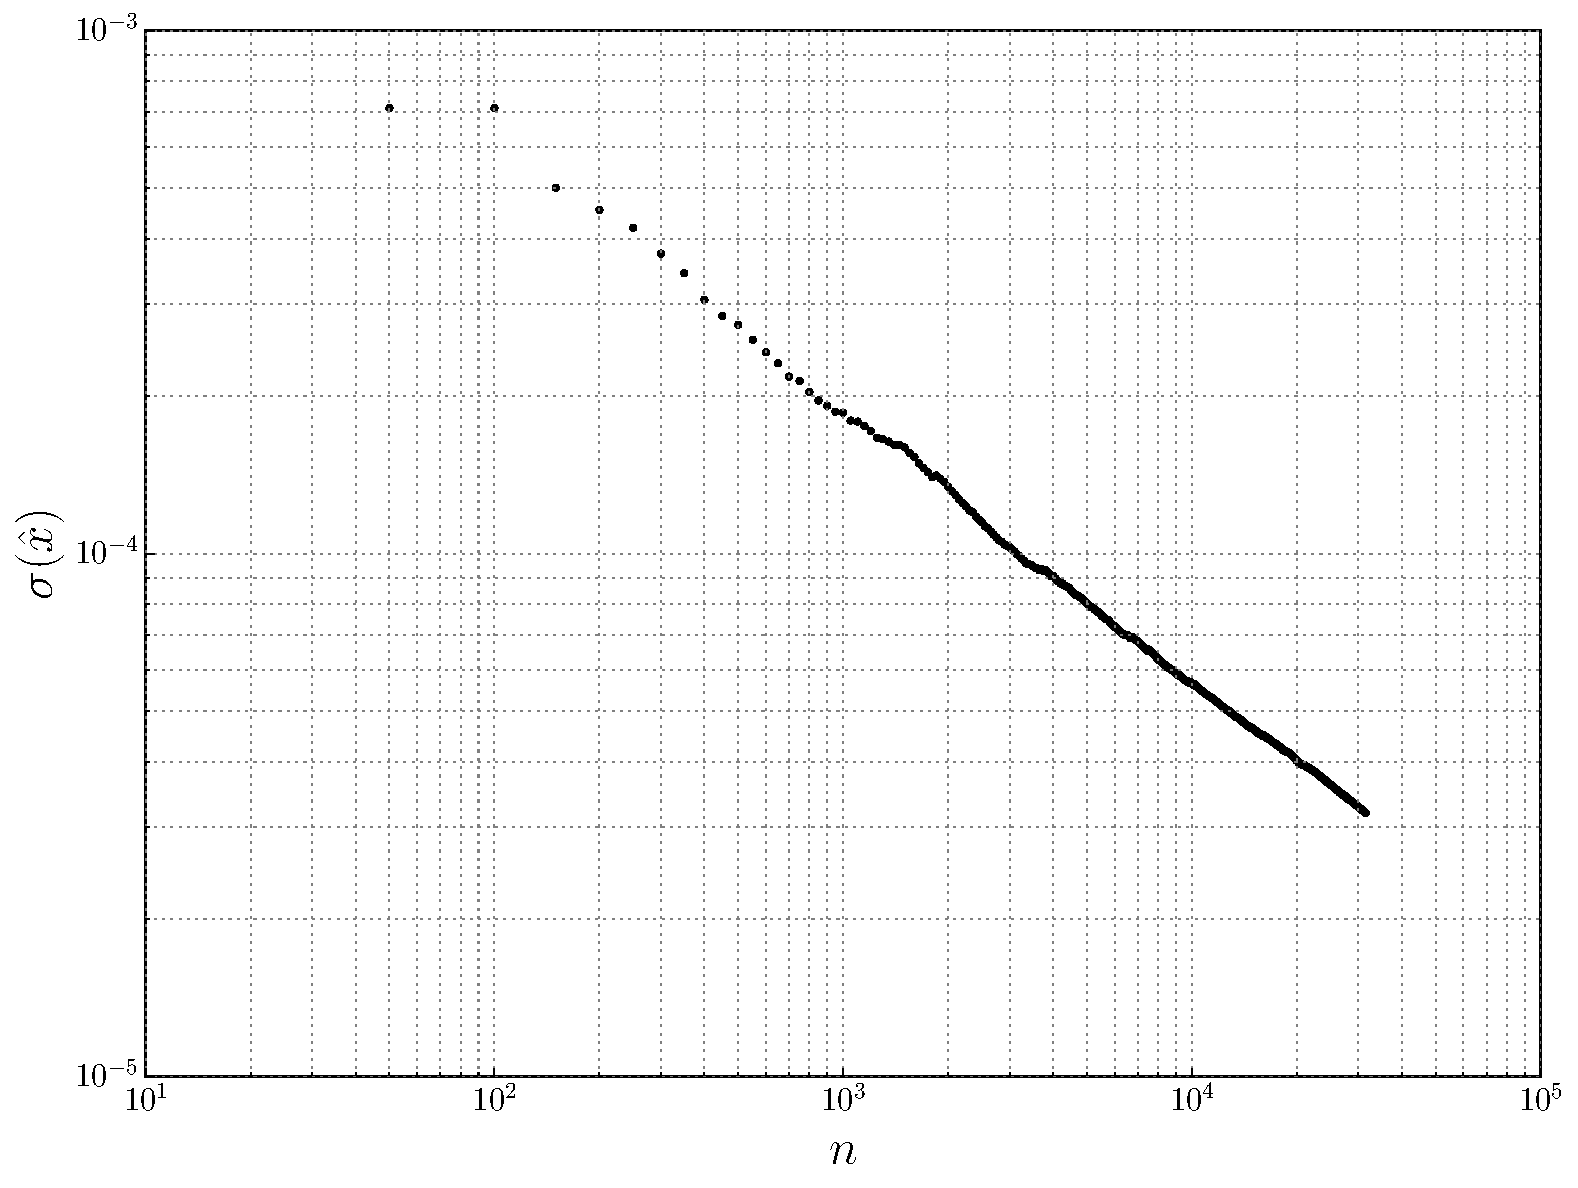
\includegraphics[scale=0.5]{images/error_convergence}
  \caption[Variance in $\phi_{\infty}$ for the fast-neutron group as a
    function of Serpent 2 cycle.]{Variance in $\phi_{\infty}$ for the fast-neutron group as a
    function of Serpent 2 cycle, with \gls{wdt} threshold of 0.2.}
  \label{fig:error_convergence}
\end{figure}
We can always reduce the variance by running the simulation longer; a
measure of our simulation quality, therefore, should be independent of
cycles. We establish a \gls{fom} that is independent of $n$.  The
standard \gls{fom} used by most simulations, described by Lewis and
Miller~\cite{lewis1993}, is shown in Eq.~\eqref{eq:fom}:
\begin{equation}
  \label{eq:fom}
  \mathrm{FOM} = \frac{1}{\sigma(\hat{x})^2T}
\end{equation}
where $T$ is the runtime of the simulation, proportional to the number
of cycles $T \propto n$. Plugging this and
Eq.~\eqref{eq:variance} into Eq.~\eqref{eq:fom}:
\begin{equation*}
  \mathrm{FOM} = \frac{1}{\sigma(\hat{x})^2T} =
  \frac{n}{C_1}\cdot\frac{1}{C_2\cdot n} = C_3
\end{equation*}
where $C_1,C_2,C_3$ are constants. As we can see, we expect the
\gls{fom} to be a constant value, independent of the number of cycles
$n$.  A higher \gls{fom} indicates higher accuracy per computation
time, and therefore a more efficient algorithm. Serpent 2 collects
scores for each cycle (or batch of cycles) and outputs the sample mean
and standard deviation~\cite{VTT-R-00371-14}. This enables comparison of Serpent 2
running with and without \gls{wdt} to determine the efficiency of the
algorithm.

\subsection{Convergence}
\label{sec:convergence}

As discussed in the previous section, the \gls{fom} should be
independent of cycle number $n$. In reality, it takes enough cycles
for good statistics to develop for the \gls{fom} to converge to its
final value. As seen in Fig.~\ref{fig:fom_convergence}, the \gls{fom}
begins to converge around $1\times 10^4$ cycles in this example. Statistical
variations in the standard deviation seen in
Fig.~\ref{fig:error_convergence} are amplified by squaring and
inverting to calculate \gls{fom}.
\begin{figure}[hbtp]
  \centering
  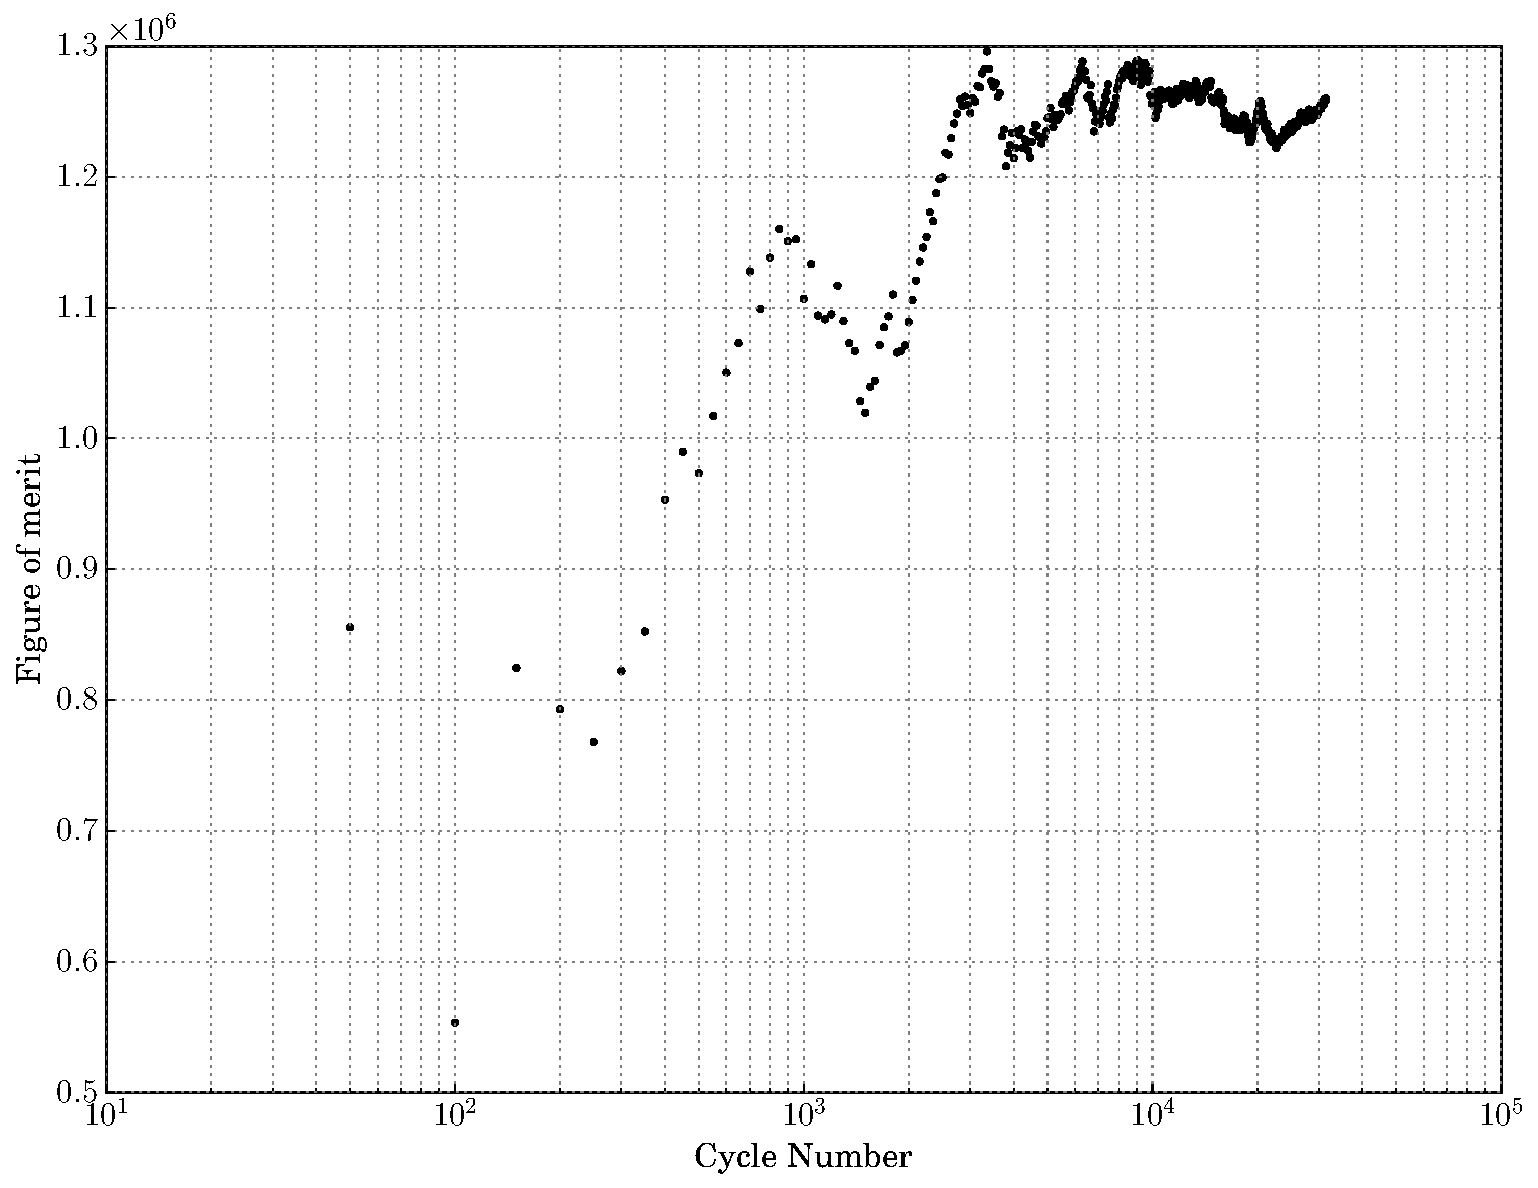
\includegraphics[scale=0.5]{images/fom_convergence_example}
  \caption[Figure of merit in $\phi_{\infty}$ for the fast-neutron group as a
    function of Serpent 2 cycle.]{Figure of merit in $\phi_{\infty}$ for the fast-neutron group as a
    function of Serpent 2 cycle, with \gls{wdt} threshold of 0.2.}
  \label{fig:fom_convergence}
\end{figure}

\subsection{Analysis Technique}
\label{sec:analysis}

Serpent 2 generates a single output file as the simulation runs. The
parameters of interest are overwritten as their mean value and
standard deviation are updated. This is sufficient to calculate the
final value of the \gls{fom} which gives an indication of the quality
of the simulation. In addition to this, figures such as those shown in
Sec.~\ref{sec:fom} are useful to verify that the \gls{fom} has in fact
converged, and that the variance is reducing as expecting. Therefore,
in addition to changing the Serpent 2 source code to include the
\gls{wdt} method, it was modified to generate uniquely named output
files at the end of each batch. Processing these files enables us to
generate to above graphs.

As seen in Fig.~\ref{fig:fom_convergence}, the final \gls{fom} is not
a single value, but may oscillate for a large number of
cycles. Therefore, we calculated an average \gls{fom} value for each
run, to allow comparison of runs without requiring a visual inspection
of each graph.

% Test Cases

\section{Test Cases}
\label{sec:test_cases}

Three test cases were used 

%% PWR
%% Fast Pincell
%% Homog Element

%% -- Images

% Actual Results

%% Infinite flux

%% Cross-sections

%% Scattering matrices

%%% Local Variables:
%%% mode: latex
%%% TeX-master: "../masters_report"
%%% End:
